\documentclass[11pt,a4paper]{article}
\usepackage[utf8]{inputenc}
\usepackage{hyperref}
\usepackage{authblk}
\usepackage{color}
\usepackage{fullpage}

\usepackage{caption}

\usepackage{booktabs}
\usepackage{lscape}

\usepackage{tikz}
\usetikzlibrary{bayesnet}
\usepackage{graphicx}
\usepackage{amsfonts}
\usepackage{amsmath,bm}
\usepackage{enumitem}
\usepackage[linesnumbered,ruled,vlined]{algorithm2e}

\usepackage{babel}

\usepackage{graphicx}
\graphicspath{ {./images/} }

\usepackage{minted}
\usepackage{tabularx}

\usepackage[
backend=biber,
style=nature,
citestyle=nature
]{biblatex}

\addbibresource{references.bib} %Imports bibliography file

\renewcommand{\topfraction}{.85}
\renewcommand{\bottomfraction}{.7}
\renewcommand{\textfraction}{.15}
\renewcommand{\floatpagefraction}{.3}
\renewcommand{\dbltopfraction}{.3}
\renewcommand{\dblfloatpagefraction}{.3}
\setcounter{topnumber}{9}
\setcounter{bottomnumber}{9}
\setcounter{totalnumber}{20}
\setcounter{dbltopnumber}{9}

\usepackage{color}
\newcommand{\red}{\textcolor{red}}
\newcommand{\blue}{\textcolor{blue}}

\hyphenpenalty=5000

\title{Comprehensive mapping of tissue cell architecture via integrated single cell and spatial transcriptomics: cell2location model \\
Supplementary Methods
}

\author{Vitalii Kleshchevnikov, Artem Shmatko, Emma Dann, Alexander Aivazidis, Hamish W King, Tong Li, Artem Lomakin, Veronika Kedlian, Mika Sarkin Jain, Jun Sung Park, Lauma Ramona, Liz Tuck, Anna Arutyunyan, Roser Vento-Tormo, Moritz Gerstung, Louisa James, Oliver Stegle, Omer Ali Bayraktar}
\date{6 November 2020}

\begin{document}

\maketitle

\tableofcontents

\section{Mapping cell types with cell2location model}

\subsection{Cell2location model} \label{cell2location_model}

Cell2location is a Bayesian model that is aimed at decomposing location-level gene expression counts into a set of pre-defined reference signatures of cell types. A representation as graphical model is shown in Fig \ref{fig:graphical_model}. The input data of the method are as follows: \newline

Let $D=\{d_{s,g}\}$ be a $S \times G$ untransformed and unnormalised spatial expression count matrix for locations $s=\{1,..,S\}$ and genes $g=\{1,..,G\}$. For 10X Visium data, this matrix can be directly obtained from the 10X SpaceRanger software and imported into data format used in a popular python package Scanpy \autocite{wolf_scanpy_2018} (see main text Methods). $D_{s,g}$ should be filtered to a set of genes expressed in the single cell reference $g_{f,g}$. Our package is interfaced with Scanpy to take advantage of their data handling and visualisation tools. For other technologies, such as Slide-Seq V2, files with count matrices of the appropriate formats need to be generated and imported into Scanpy data format by the user. \newline

Let $G=\{g_{f,g}\}$, denote an $F \times G$ matrix of reference signatures of cell types, which consist of $f=\{1,..,F\}$ reference signatures, each of which is defined by a gene expression profile $G_{f,:}$ for $g=\{1,..,G\}$ genes. This matrix needs to be provided to cell2location and can be estimated from scRNA-seq profiles. Strategies how to estimate this matrix are presented in Section \ref{c2l_ref_prog}. \newline
Using a cell type reference from the same tissue specimen provides the benefit of knowing the exact expression signatures of cell types present in the spatial tissue section. When an unmatched cell type reference is used, cells located \emph{in-situ} might have a different state (such as metabolic activation) or regional signature, so cell2location will map the most similar cell type (metabolically inactive cells) from the reference in place of the true cell type (metabolically active cells). \newline

\begin{figure}
    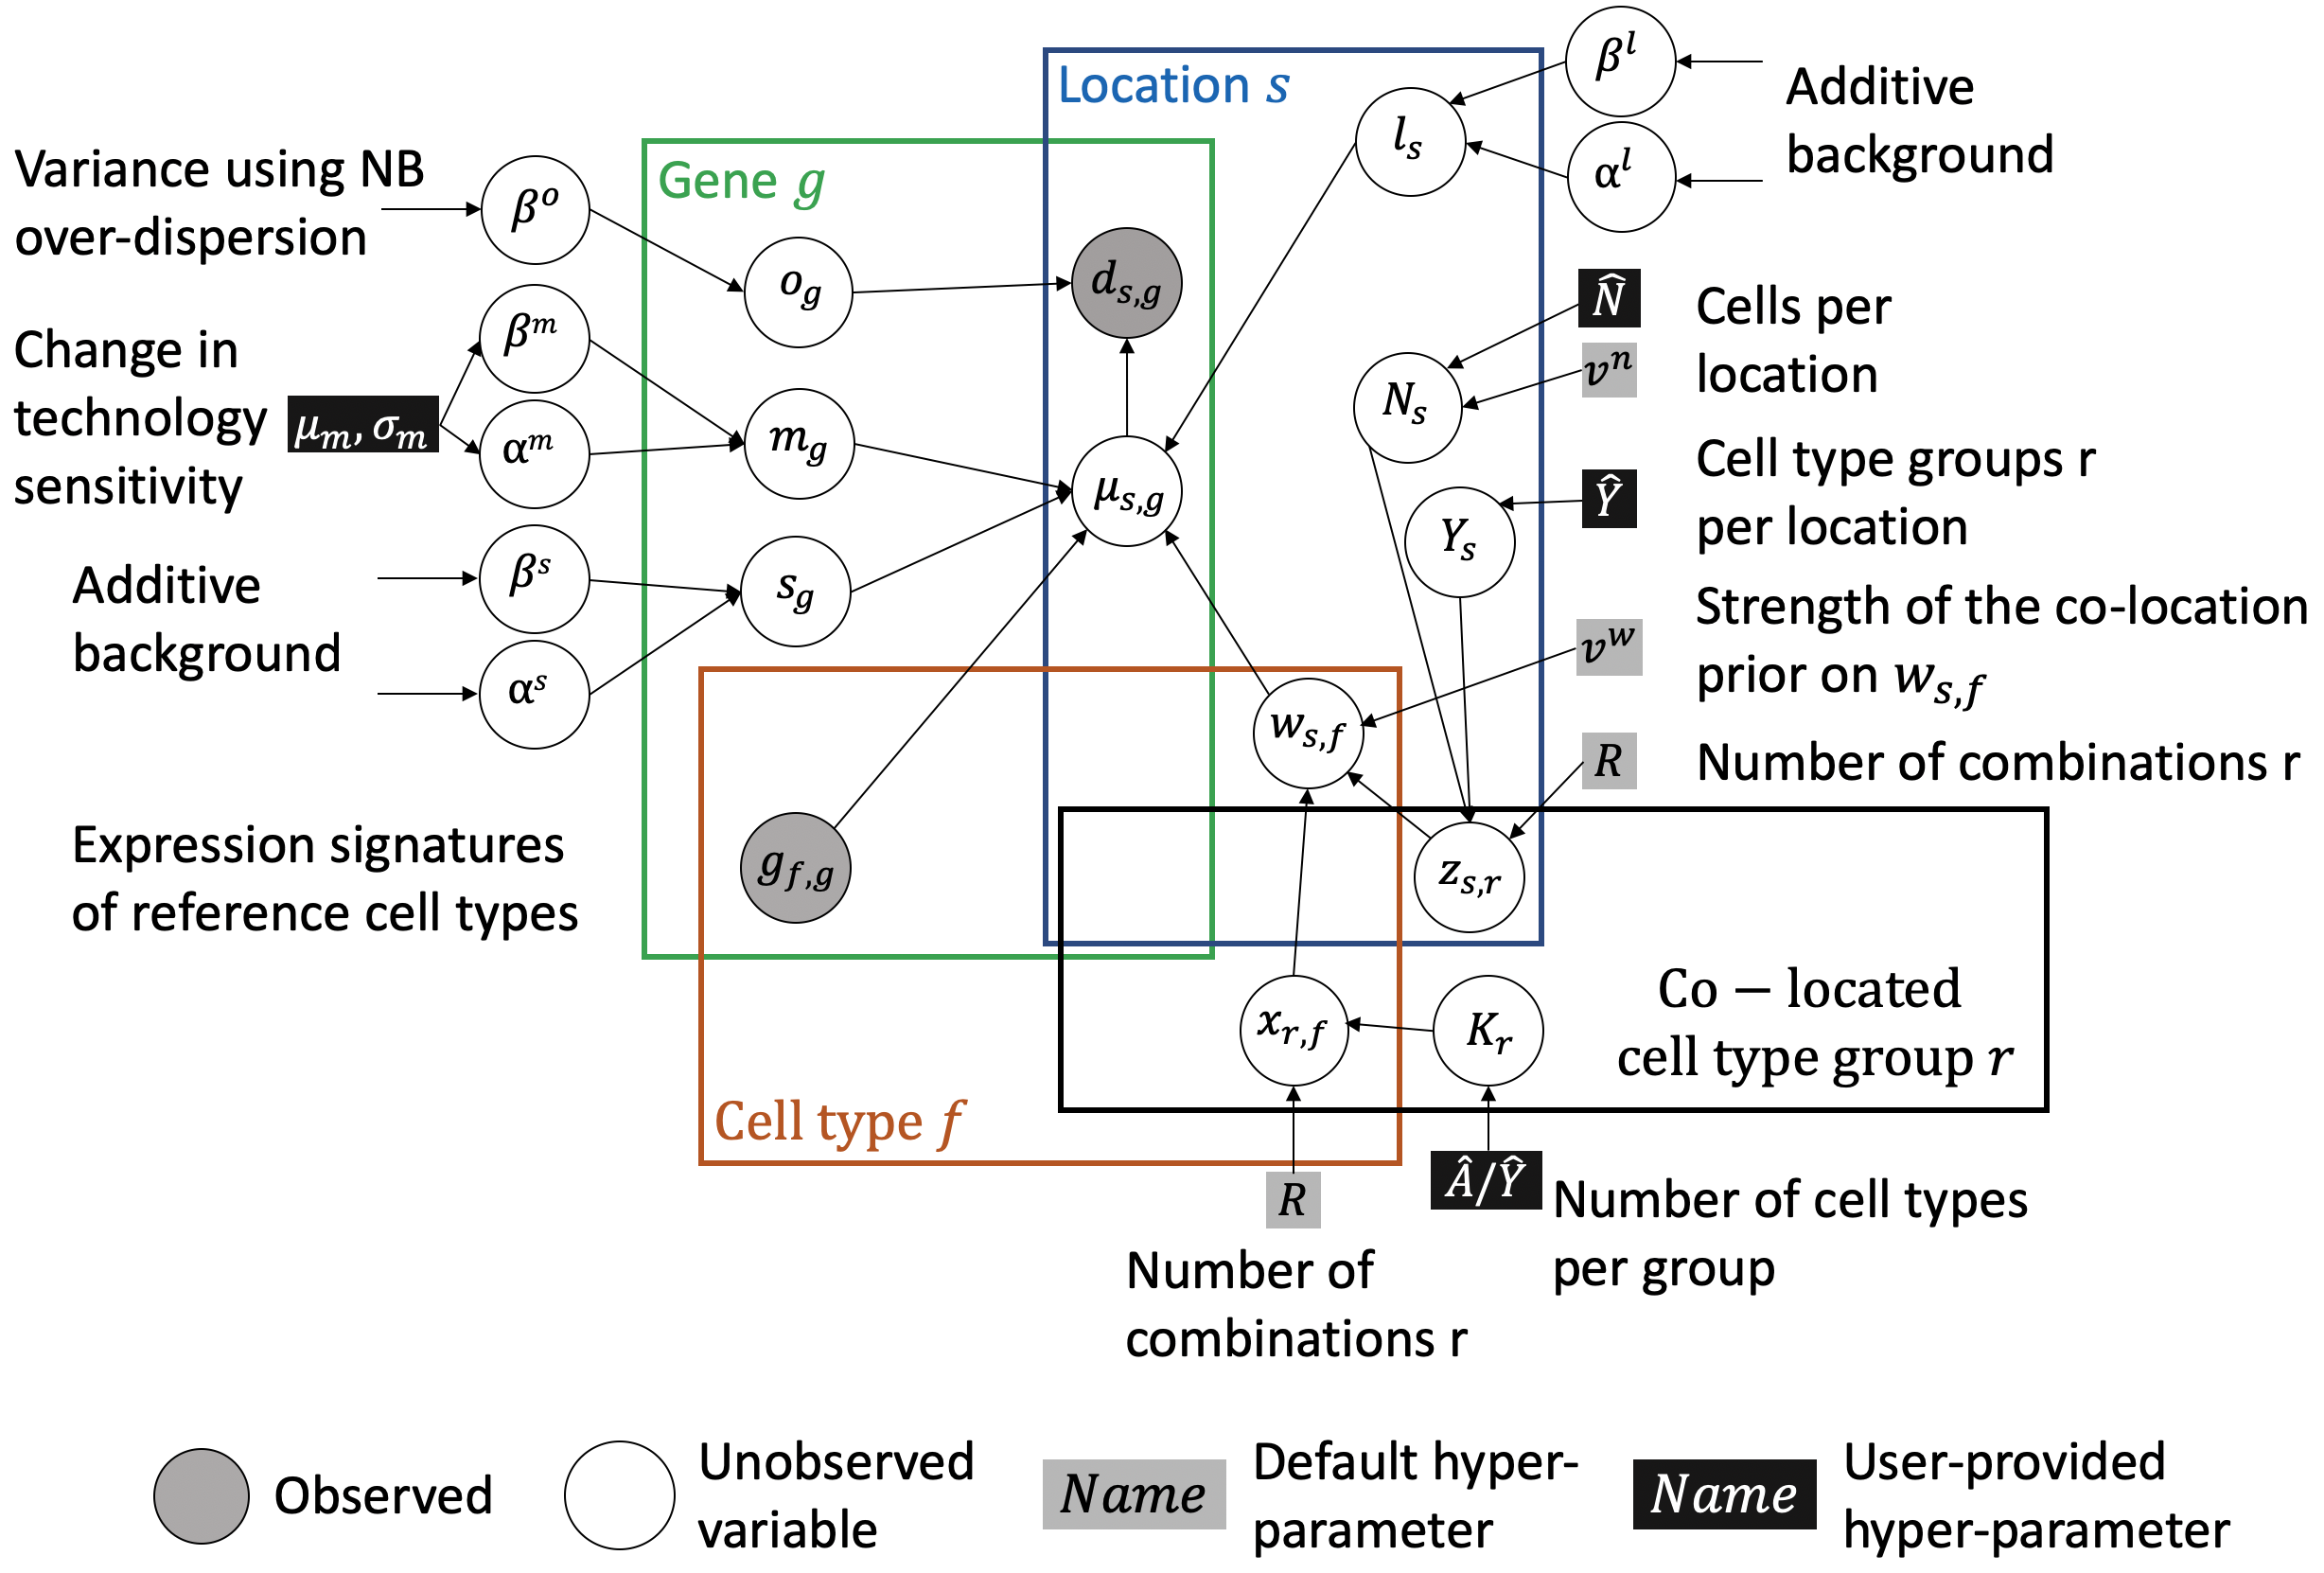
\includegraphics[scale=0.4]{images/LocationModelLinearDependentW.png}
    \caption{Illustration of the corresponding graphical model.}
    \label{fig:graphical_model}
\end{figure}

Cell2location models the elements of $D$ as Negative Binomial distributed, given an unobserved expression level (rate) $\mu_{s,g}$ and a gene-specific over-dispersion parameter $\alpha_g$ which accounts for variance in expression of individual genes that is not explained by the reference signatures of cell types: 
\begin{equation} \label{eq:c2l:1}
D_{s,g} \sim \mathtt{NB}(\mu_{s,g}, \alpha_g) \\
\end{equation}

Note that this is equivalent to a Poisson variable (measurement model) with a Gamma-distributed mean (expression model)
\autocite{sarkar_separating_2020}. Here NB distribution is parameterised by $\mu$ and over-dispersion $\alpha$, also called $\theta$, which corresponds to shape parameter of Gamma distribution in Gamma-Poisson mixture.
\begin{equation} \label{eq:c2l:1}
D_{s,g} \sim \mathtt{Poisson}(\mathtt{Gamma}(\alpha_g, \alpha_g / \mu_{s,g})) \\
\end{equation}

The expression of level of genes $\mu_{s,g}$ in the rate space is modelled as a linear additive additive decomposition:
\begin{equation} \label{eq:c2l:3}
\mu_{s,g} = m_{g} \left (\sum_{f} {w_{s,f} \: g_{f,g}} \right) + l_s + s_{g}\\
\end{equation}

Here, $w_{s,f}$ denotes regression weight of each reference signature $f$ at location $s$; 
$m_{g}$ denotes a gene-specific scaling parameter to account for global differences in expression estimates between technologies;
$l_{s}$ and $s_{g}$ are gene- and location-specific additive components that capture additive background variation that is not explained by reference cell type signatures. \\

The prior distributions on the unobserved parameters are as follows:
\begin{enumerate}
    \item \textbf{Absolute abundance of cell types across locations.}
    The regression weights $w_{s,f}$ for each reference signature, which can be interpreted as the number of cells per location $s$ expressing each each reference signature $f$, are Gamma distributed and referred to in the cell2location software as \mintinline{python}|'spot_factors'|. \newline
    \begin{equation} \label{eq:c2l:4}
    w_{s,f} \sim \mathtt{Gamma}(mu = {\mu}^{w}_{s,f}, \sigma^2 = {\mu}^{w}_{s,f} / v^{w})
    \end{equation}
    where the scalar constant $v^{w}$ controls the extent to which this co-abundance prior $\mu^{w}_{s,f}$ controls $w_{s,f}$.
    
    The mean parameter of this distribution ${\mu}^{w}_{s,f}$ is modelled using another layer of decomposition into the latent groups of cell types $r=\{1,..,R\}$ to account for linear dependencies in spatial abundance of reference signatures $f$, where $R$ is specified by the user:
    
    \begin{equation} \label{eq:c2l:5}
    {\mu}^{w}_{s,f} = \sum_{r} {z_{s,r} \: x_{r,f}}\\
    \end{equation}
    
    The groups of cell types can be thought of as cellular compartments in the tissue. As illustrated by validation on simulated data (Fig S2A), modelling these linear dependencies increases the sensitivity of cell2location for mapping cell types at low abundance in particular. Note this model is not using spatial coordinates or proximity of locations. The rationale behind this decision is that expression can change abruptly in spatial coordinates, with neighbouring locations having distinct cell composition (Fig S16A). Also, since the model does not make use of coordinates to estimate $w_{s,f}$, coordinates can be used in downstream analysis to validate spatial patterns in $w_{s,f}$ estimates.
    
    The prior distributions of $z_{s,r}$ and $x_{r,f}$ are defined to control absolute scale of the cell type abundance estimates $w_{s,f}$, to enable interpretation as the number of cells per location $s$ expressing each cell type reference signature $f$. In addition, these prior distributions control the sparsity of how many cell types $f$ are present in each location $s$, enabling application of cell2location to tissues and technologies with varying numbers of cells and cells types per location.
    
    \begin{itemize}
        \item The total spatial abundance $z_{s,r}$ of latent cell type groups $r$ across locations $s$ is defined as Gamma distributed with a prior controlling the scale and sparsity of this distribution:
        \begin{equation} \label{eq:c2l:6}
        z_{s,r} \sim \mathtt{Gamma}(Y_s / R, 1 / (N_s / Y_s))
        \end{equation}
    
        where $N_s$ is the average number of cells in each location, and $Y_s$ is the number of latent groups $r$  present in each location $s$ - which are both unobserved but depend on user input (See eq.~\eqref{eq:c2l:7}-\eqref{eq:c2l:8} and  section \ref{hyper-parameters}). The prior on $z_{s,r}$ is specified such that $\sum_{r} z_{s,r}$ on average equals to the number of cells per location $\sum_{r} z_{s,r} = N_s$, and that on average each location has high $z_{s,r}$ for $Y_s$ cell type groups. 
        
        Unobserved $Y_s$ and $N_s$ parameters are modelled as Gamma-distributed:
        \begin{equation} \label{eq:c2l:7}
        N_s \sim \mathtt{Gamma}(mu=\hat{N}, \sigma^2=\hat{N} / v^{n})
        \end{equation}
        \begin{equation} \label{eq:c2l:8}
        Y_s \sim \mathtt{Gamma}(mu=\hat{Y}, \sigma^2=\hat{Y})
        \end{equation}
        where $\hat{N}$ is a user-provided rough estimate of the number of cells per location; $\hat{Y}$ is a user-provided average number of cellular compartments / zones per location; and $v^{n}$ is measure of uncertainty in $\hat{N}$ estimates. Recommendation on setting there hyper-parameters are outlined in section \ref{hyper-parameters}.
        
        \item The latent variable $x_{r,f}$ represents the contribution of each latent cell type group $r$ to the abundance of cell types $f$ and is Gamma distributed with a prior controlling the number of cell types $f$ that have high values of $x_{r,f}$ in each group $r$:
        \begin{equation} \label{eq:c2l:10}
        x_{r,f} \sim \mathtt{Gamma}(K_r / R, K_r)
        \end{equation}
        where $K_r$ represents the unobserved number of cell types for each group $r$. Under this prior $\sum_{r} x_{r,f} = 1$.
        
        $K_r$ is Gamma-distributed with a prior informed by user input:
        \begin{equation} \label{eq:c2l:11}
        K_r \sim \mathtt{Gamma}(mu =  \hat{A} / \hat{Y}, \sigma^2 = \hat{A} / \hat{Y})
        \end{equation}
        where $\hat{A}$ is a user-provided average number of cell types per location; and $\hat{Y}$ is a user-provided average number of cellular compartments / zones per location (See recommendations in section \ref{hyper-parameters}). This prior tells that each group $r$ has large $x_{r,f}$ for many cell types $f$ when $\hat{A} > \hat{Y}$, and $\hat{A} = \hat{Y}$ indicates that the spatial abundance of each cell type $f$ is independent from other cell types. 
    
        \end{itemize}
    
    \item \textbf{Gene-specific multiplicative scaling factor} $m_{g}$ is modelled as Gamma-distributed (Eq. \eqref{eq:c2l:12} - \eqref{eq:c2l:14}) with hierarchical prior $\alpha^m$ and $\beta^m$ reflecting the prior belief about the difference in sensitivity of single cell and spatial technologies. This way we are not assuming certain change in sensitivity but allowing the model to learn it.
    \begin{equation} \label{eq:c2l:12}
    m_{g} \sim \mathtt{Gamma}(\alpha^m, \beta^m) 
    \end{equation}
    \begin{equation} \label{eq:c2l:13}
    \alpha^m \sim \mathtt{Gamma}(mu = \mu_m ^ 2 / \sigma_m ^ 2, \sigma^2 = \mu_m ^ 2 / \sigma_m ^ 2)
    \end{equation}
    \begin{equation} \label{eq:c2l:14}
    \beta^m \sim \mathtt{Gamma}(mu = \mu_m / \sigma_m ^ 2, \sigma^2 =\mu_m / \sigma_m ^ 2)
    \end{equation}
    
    where $\mu_m$ is an average change in sensitivity, $\sigma_m$ describes the deviation of the sensitivity of individual genes from $\mu_m$. The link between these hyper-parameters and priors $\alpha^m, \beta^m$ is set as described in the notation section \ref{Notation}. Section \ref{hyper-parameters} details how these hyper-parameters are derived from data.
    
    \item \textbf{Additive background for genes and locations.} $l_s$ and $s_{g}$ are modelled as Gamma distributed with hierarchical priors on shape and rate of their distributions eq.~\eqref{eq:c2l:15} - \eqref{eq:c2l:19}:
    \begin{equation} \label{eq:c2l:15}
    l_s \sim \mathtt{Gamma}(\alpha^l,  \beta^l)
    \end{equation}
    \begin{equation} \label{eq:c2l:18}
    s_{g} \sim \mathtt{Gamma}(\alpha^s,  \beta^s)
    \end{equation}
    \begin{equation} \label{eq:c2l:19}
    \alpha^l, \beta^l, \alpha^s, \beta^s \sim \mathtt{Gamma}(1, 1)
    \end{equation}
    
    \item \textbf{Overdispersion for each gene.} Containment prior \autocite{simpson_penalising_2017} is used for modelling unobserved variance using NB over-dispersion $\alpha_g$. The idea of a containment prior is that, by the prior, NB distribution should be maximally close to Poisson distribution, which is achieved by putting most probability mass on large $\alpha_g$. So, under the following prior most genes have low over-dispersion:
    \begin{equation} \label{eq:c2l:21}
    \alpha_g = 1 / o_g ^ 2
    \end{equation}
    \begin{equation} \label{eq:c2l:22}
    o_g \sim \mathtt{Exponential}(\beta^o)
    \end{equation}
    \begin{equation} \label{eq:c2l:23}
    \beta^o \sim \mathtt{Gamma}(mu, \sigma^2)
    \end{equation}
    where constants $mu$ and $\sigma^2$ are provided by the user (See section \ref{hyper-parameters}).

\end{enumerate}


In addition to reporting absolute cell density we also compute absolute number of mRNA molecules ($u_{s,f}$) contributed by each cell type $f$ to each location $s$:
\begin{equation} \label{eq:c2l:24}
u_{s,f} = w_{s,f} (\sum_{g} {m_{g} \: g_{f,g}})
\end{equation}
These parameters are referred to in the package as \mintinline{python}|'nUMI_factors'|. $u_{s,f}$ are a more robust estimate than either absolute cell density $w_{s,f}$ or relative cell proportions $w_{s,f} / \sum_{f} w_{s,f}$. For this reason it can be used as a criteria to accurately exclude non-mapped cell types (Fig S9). \newline

\subsection{Multi-experiment extension of cell2location model} \label{c2l_multi}

When analyzing multiple spatial data sets jointly, where $e=\{1,..,E\}$ denote individual experiments, such as 10X Visium square capture area and Slide-Seq V2 ``puck", the over-dispersion parameter $\alpha_{e,g}$ and additive background parameter $s_{e,g}$ are fit separately for each experiment as well as genes. Specifically, $\alpha_{e,g}$ depends on $o_{e,g}$ which is modelled as independent and exponentially distributed (eq.~\eqref{eq:c2l:1multi} - \eqref{eq:c2l:2multi}) and $s_{e,g}$ is modelled as iid Gamma (eq.~\eqref{eq:c2l:3multi}):
    \begin{equation} \label{eq:c2l:1multi}
    D_{s,g} \sim \mathtt{NB}(\mu_{s,g}, \alpha_{e,g} = 1 / o_{e,g} ^ 2) \\
    \end{equation}
    \begin{equation} \label{eq:c2l:2multi}
    o_{e,g} \sim \mathtt{Exponential}(\beta^o)
    \end{equation}
    \begin{equation} \label{eq:c2l:3multi}
    s_{e,g} \sim \mathtt{Gamma}(\alpha^s,  \beta^s)
    \end{equation}
Individual locations belong to experiments, $s \in e$, therefore only the following variables are shared between experiments:
\begin{enumerate}

    \item $g_{f,g}$, the same reference cell type signatures are used for all experiments.
    
    \item $m_{g}$, the change in sensitivity between technologies is shared across experiments, improving the ability of the model to distinguish low $m_{g}$ from zero cell abundance $w_{r,f}$. This is equivalent to regressing out the effect of technology but not the effect of individual experiment. 
    
    \item $x_{r,f}$, the latent groups $r$ of reference cell types $f$ with similar spatial abundance, and it's hierarchical prior, $N_r^{x}$, the number of cell types per group
    
    \item Variables that serve as hierarchical priors (single value for each variable): $\alpha^m$, $\beta^m$, $\alpha^l$, $\beta^l$, $\alpha^s$, $\beta^s$, $\beta^o$
    
\end{enumerate}

\subsection{Selecting hyper-parameters} \label{hyper-parameters}

Unless stated otherwise, we use the following strategy to The following priors need to be adjusted by the user to every tissue and technology:
\begin{enumerate}
    \item Cell number $\hat{N}$ per location can be estimated from paired histology images and from size of capture regions relative to the size of cells. Note, that the model does not require knowing the exact number of cells obtained by counting nuclei in each location. 
    
    Advanced usage. When the cell count, obtained by segmenting histology data paired with $D_{s,g}$ for each location $s$, is available it can be provided as a location-specific $\hat{N_s}$ parameter and $v^{n}$ can be adjusted to make the prior more informative ($v^{n}=10$). When the size of cell capture areas varies, such as in laser capture microscopy (LCM) method, we recommend to use a location-specific $\hat{N_s}$ parameter.
    \item The number of cell types $\hat{A}$ can be chosen based on the complexity of the tissue: number of cell types in the reference, number of cells per location $\hat{N}$, whether locations are dominated by a single cell type, and the size of capture areas. 
    \item The number of tissue zones $\hat{Y}$ per location can based on complexity of the tissue: presence of spatially interlacing tissue zones (high complexity), discrete regions with dominant cell types (low complexity). The number of zones equal to the number of cell types reflects a prior belief that cell type location patterns are independent (do not resemble each other).
    \item Average difference in technology sensitivity $\mu_m$ and $\sigma_m$ parameters in eq.~\eqref{eq:c2l:13}-\eqref{eq:c2l:14} are chosen by comparing average total number of mRNA per cell in the reference cell type data and the average total number of mRNA per location in the spatial data divided by $\hat{N}$. This process will be automated in future versions of cell2location.
\end{enumerate}

The model will give more accurate absolute cell abundance estimates when these priors are chosen well. We observed 5-6 cell types and 8 cells per location in the mouse brain 10X Visium (Fig S6, Fig S10), but just 1-2 cell types and cells in the human brain and heart (unpublished, using published spatial data). In the lymphoid and epithelial tissues, 10X Visium locations contain about 10 cell types and 30 cells per location reflecting high spatial interlacing of cell type locations in these tissues (Fig S10 and unpublished). Slide-Seq V2 locations have 1-2 cell types and fractions of cells in each location (Fig S10). We also note that we observed large absolute cell abundance $w_{s,f}$ in the Slide-Seq V2 data (Fig 2H) potentially indicating that additional technical effects such as difference in sensitivity between beads need to be accounted for. \newline


The following priors are used at their default values:
\begin{enumerate}
    \item The number of co-located cell type groups is $R=50$ by default. The model tends to find 3-7 groups $r$ with substantial values of $x_{r,f}$.
    \item Hyper-paramter $v^w$, controlling the extent to which the co-abundance prior controls $w_{s,f}$, is set to a medium value of $v^w=5$. Increasing $v^w$ forces stronger linear dependencies in $w_{s,f}$ leading to over-smoothing and lower model accuracy. Decreasing $v^w$ leads to cell types $f$ modelled as independent, such that given the extent of those effects are in real data, this also decreases model accuracy.
    \item $v^n$ in eq.~\eqref{eq:c2l:8} is set to 1 when a global rather than location-specific estimate $\hat{N}$ is specified.
    \item Constants $mu=3$ and $sd=1$ in eq.~\eqref{eq:c2l:23} are chosen to scale the exponential distribution in eq.~\eqref{eq:c2l:22} to put most probability density at low over-dispersion (large $\alpha_g$). The inference of this parameter appears to be fairly robust to the choice of $mu$ and $sd$. Nonetheless, the estimate of $\beta^o$ is substantially different between single cell and single nucleus data sets.
\end{enumerate}

\subsection{Inference} \label{c2l_inference}

Variational Bayesian Inference is used to approximate the posterior, specifically black-box Automatic Differentiation Variational Inference (ADVI) implemented in pymc3 framework \autocite{salvatier_probabilistic_2016}. Appropriately transformed (to positive scale) univatiate normal distributions are used to approximate each parameter. Inference is achieved by maximising log-likelihood of the data and minimising KL divergence from the posterior to prior, which are combined in the evidence lower bound (ELBO loss function). Training is stopped when ELBO stops increasing, usually after 20 000 - 40 000 iterations of training using ADAM optimiser (learning rate 0.005) with gradient clipping (total gradient norm $<$ 200). Posterior mean, standard deviation, 5\% and 95\% quantiles for each parameter where computed using 1000 samples from the Variational posterior distribution. We observed that 5\% quantile provides a marginally more accurate estimate of cell abundance compared to the mean (not shown). 


Two or more restarts are performed to evaluate the stability of the inferred posterior distribution, but under default parameters inference is very stable so no selection of the best model is performed (the first training restart is used). Yet, it is an important quality control step, with divergences between restarts reflecting poor match of the cell type reference or large mismatch between the prior distribution of $D_{s,g}$ (sample from the model given hyper-parameter choices) and the count distribution in the observed data $D_{s,g}$ (prior predictive check). Validity of selected hyper-parameters is evaluated using prior predictive check (also provided within the package) but this step is not essential for 10x Visium data sets where the model showed good performance. For every analysis, performance of the training is evaluated, as shown in \href{https://cell2location.readthedocs.io/en/latest/notebooks/cell2location_short_demo.html#Evaluating-training}{\blue{the tutorial}}: 1) by comparing the posterior mean estimate $log10(\mu_{s,g} + 1)$ to observed data $log10(D_{s,g} + 1)$ (posterior predictive check); 2) by evaluating consistency of inferred $w_{s,f}$ parameters between the training restarts.

\subsection{Nuclei Segmentation (optional)} \label{c2l_segmentation}

To perform nuclei segmentation, H\&E-stained image of the Visium-profiled tissue was used. The image was acquired using Hamamatsu slide scanner as described in the section on experimental processing. Full resolution images were divided into sub-images of size about 1000 by 1000 pixels. Then a state-of-the-art convolutional neural network (CNN)-based segmentation pipeline described in Caicedo et al.~\autocite{caicedo_nucleus_2019} and available in GitHub repository \href{https://github.com/selimsef/dsb2018_topcoders}{\blue{selimsef/dsb2018\_topcoders}} was used. An ensemble of 32 pre-trained CNNs each with Unet- or FPN-like architecture was used to classify pixels to 3 classes: background, nuclei and nuclei boundaries. Predicted segmentation masks were averaged across CNNs, then a watershed algorithm was applied to refine predicted boundaries and separate individual nuclei. As a final step, a gradient boosting model over morphological features such as nuclei colour, shape and size was used to remove false-positively detected nuclei.  
Obtained individual nuclei masks were used to compute several morphological features: 1) area (count of pixels in a mask), 2) shape - ratio of lengths of the major and minor axis of an ellipse fitted to the mask, and 3) position - center of mass of the image containing individual mask.
Kd-tree approach was used to efficiently assign nuclei to Visium locations. Kd-tree implementation from the scikit-learn package was used. Nuclei positions in the histology image are reported in Suppl.~Data.

\section{Estimation of reference expression signatures of cell types} \label{c2l_ref_prog}

We obtain reference expression signatures of cell types $G_{fg,}$ from scRNA-seq  expression data $J=\{j_{c,g}\}$ of each gene $g=\{1..G\}$ in cell $c=\{1..C\}$. First, untransformed and unnormalised count matrix $J_{c,g}$ is filtered to select expressed genes (Fig S1) at 2 cut-offs: 1) selecting genes detected at mRNA count $>$ 0 in many cells ($>$ 5\% of cells), 2) selecting genes detected at mRNA count $>$ 0 in a few cells (5\% $>$ cell count $>$ 10) but with large mean expression across non-zero cells ($>$ 1). Next, we use following 2 alternative methods to compute $g_{f,g}$,however, whenever possible 2nd method should be used:
\begin{enumerate}
    \item \textbf{Cell type references produced by a single experiment.} Analytically computing single cell reference cluster centroids for each gene $g$ and cell cluster $f=\{1..F\}$. This method is very computationally efficient and gives very good mapping quality (measured on simulated data) when the scRNA-seq reference is a single sample matching the source of spatial data $D_{s,g}$, or a few samples with no strong batch effect between them. We also use this methods for Smart-Seq 2 scRNA-seq data because the second method needs to be extended to utilise this data type.
    \item \textbf{Complex cell type references produced multiple experiments and technologies.} To address the usage of challenging reference data composed of multiple batches $e=\{1..E\}$ and technologies $t=\{1..T\}$, the biological reference expression signatures $g_{f,g}$ of each gene $g$ in each single cell reference cluster $f$ are estimated using a regularised Negative Binomial regression. The model accounts for the difference in global sequencing coverage $h_e$ between experiments, gene-specific difference in sensitivity between technologies $p_{t,g}$ and background expression $b_{e,g}$ of each gene in each experiment $e$. It models unexplained variance (over-dispersion $\alpha_g$) and count nature of the data using Negative Binomial distribution:
    \begin{equation} \label{eq:c2l_ref_prog:1}
    J_{c,g} \sim \mathtt{NB}(\mu_{c,g}, 1 / \alpha_g^2)
    \end{equation}
    \begin{equation} \label{eq:c2l_ref_prog:2}
    \mu_{c,g} = (g_{f,g} + b_{e,g}) \: {h_e} \: p_{t,g}
    \end{equation}
    All model parameters are constrained to be positive to simplify interpretation. Weak L2 regularisation of $g_{f,g}$ / $b_{e,g}$ / $\alpha_g$ and penalty for large deviations of $h_e$ and $p_{t,g}$ from 1 is used. $g_{f,g}$ is initialised at analytical average for each cell type $f$ and $b_{e,g}$ is initialised at average expression of each gene $g$ in each experiment $e$ divided by a factor of 10. Such informative initialisation leads to fast convergence.  \newline
    Pytorch implementation of training using mini batches makes the model fast (30sec-5min on GPU) and scalable to very large data sets ($>$ 100k cells). Maximum a posteriori optimisation is used to find parameters of this model with batch size of 1024 cells, ADAM optimiser learning rate 0.01. The number of epochs needed for training is determined using cross-validation performed on held-out 10 percent of cells of each cell type $f$. \newline
    To verify that the model successfully accounted to non-biological sample effects $h_e$, $p_{t,g}$ and $b_{e,g}$, a corrected expression matrix $J^{corrected}_{c,g}$ is obtained by normalising $J_{c,g}$:
    \begin{equation} \label{eq:c2l_ref_prog:3}
    J^{corrected}_{c,g} = J_{c,g} / ({h_e} \: p_{t,g}) - b_{e,g}
    \end{equation}
    $J^{corrected}_{c,g}$ matrix is subjected to standard Scanpy workflow \autocite{wolf_scanpy_2018} to verify the mixing of the cells from different samples and technologies within matching cells types (Fig S17B).

\end{enumerate}

\subsection{Differential expression between reference signatures} \label{c2l_ref_prog_diff_expression}

To identify markers of reference cell types we implemented the regression model presented in the previous section \ref{c2l_ref_prog} using a principled Bayesian framework. All model variables are constrained to be positive to simplify interpretation. The following priors are used with empirically chosen hyper-parameters:
\begin{equation} \label{eq:c2l_ref_prog_diff:3}
g_{f,g} \sim \mathtt{Gamma}(gs, gr)
\end{equation}
\begin{equation} \label{eq:c2l_ref_prog_diff:4}
gs \sim \mathtt{Gamma}(mu=0.3, \sigma^2=0.3/3)
\end{equation}
\begin{equation} \label{eq:c2l_ref_prog_diff:4}
gr \sim \mathtt{Gamma}(mu=0.8, \sigma^2=0.8/3)
\end{equation}

where $var = mu / 3$ to make the prior $mu$ more informative. The specific value of $mu$ was chosen by fitting $gs$ and $gr$ Gamma distribution parameters with pymc3 implementation of MCMC to $g_{f,g}$ obtained by maximum likelihood on mouse brain data (section \ref{c2l_ref_prog}).

\begin{equation} \label{eq:c2l_ref_prog_diff:5}
b_{eg} \sim \mathtt{Gamma}(bs, br)
\end{equation}
\begin{equation} \label{eq:c2l_ref_prog_diff:6}
bs \sim \mathtt{Gamma}(mu=0.45, \sigma^2=0.45/3)
\end{equation}
\begin{equation} \label{eq:c2l_ref_prog_diff:7}
br \sim \mathtt{Gamma}(mu=11, \sigma^2=11/3)
\end{equation}

where $\sigma^2 = mu / 3$ to make the prior $mu$ more informative. The specific value of $mu$ was chosen by fitting $bs$ and $br$ Gamma distribution parameters with pymc3 implementation of MCMC to $b_{e,g}$ obtained by maximum likelihood on mouse brain data (section \ref{c2l_ref_prog}).

Similarly to the maximum likelihood model, priors were chosen to penalise deviation of $h_e$ and $p_{tg}$ from 1, with stronger penalisation for $p_{tg}$ (10 compared to 6):
\begin{equation} \label{eq:c2l_ref_prog_diff:8}
h_e \sim \mathtt{Gamma}(6, 6)
\end{equation}
\begin{equation} \label{eq:c2l_ref_prog_diff:9}
p_{tg} \sim \mathtt{Gamma}(10, 10)
\end{equation}

Fitting of $g_{f,g}$ and $b_{e,g}$ estimates was initialised similarly to the maximum likelihood model. The Bayesian regression model is implemented in pyro \autocite{bingham_pyro_2018}, including training using mini batches, which makes model comparably scalable and fast. Optimisation is used to find Variational Posterior of the parameters with batch size of 1024 cells, ADAM optimiser learning rate 0.001. The training is stopped before $p(J_{c,g} | \mu_{c,g}, 1 / \alpha_g^2$) starts decreasing. \newline

To identify genes most specific to each reference cell type $f$, such as astrocyte sub-types, the following algorithm was applied to the posterior distribution of $g_{f,g}$:
\begin{enumerate}
    \item Normalise each sample from the posterior distribution such that $g^{norm}_{f,g} = g_{f,g} / \sum_{f} g_{f,g}$.
    \item Compute 5\% quantile of the posterior distribution of $g^{norm}_{f,g}$ to incorporate uncertainty in the estimates
    \item Rank genes for each cell type $f$ using 5\% quantiles of normalised expression $g^{norm}_{f,g}$ computed in step 2
\end{enumerate}

\section{Comparison of cell2location with existing methods} \label{comparison_of_c2l_to_other}

Table \ref{tab:table1} compares cell2location with other existing methods.


\begin{table}[h]
\hyphenpenalty=100000
\caption{Comparison of cell2location with other existing methods}
\label{tab:table1}
\renewcommand{\arraystretch}{1.35}
\resizebox{\textwidth}{!}{%
\begin{tabular}{@{} m{5cm} m{3cm} m{3cm} m{3cm} m{3cm} m{3cm} m{3cm} @{}}
\toprule
Criteria &
  cell2location &
  stereoscope \autocite{andersson_spatial_2019} &
  Seurat V3 \autocite{stuart_comprehensive_2018} &
  SpotLIGHT \autocite{elosua_spotlight_2020} &
  NNLS (autogenes) \autocite{aliee_autogenes_2020} &
  RCTD \autocite{cable_robust_2020} \\ \toprule
1.\kern.2em Data\kern.3emdistribution, normalisation &
  Negative Binomial, non-negative parameters &
  Negative Binomial, non-negative parameters &
  Normalised log(x+1) &
  Counts, non-negative parameters &
  Counts, non-negative parameters &
  Negative Binomial, log-normal model \\ \hline
2.\kern.2em Inference method &
  Variational Inference &
  Penalised maximum likelihood &
  PCA + MNN &
  NNLS &
  NNLS &
  Penalised maximum likelihood \\ \hline
3.\kern.2em Accounting for the difference in sensitivity between single cell and spatial technology &
  Yes &
  Yes &
  Unclear &
  No &
  No &
  Yes, but less flexible than cell2location and stereoscope \\ \hline
4.\kern.2em Modelling linear dependencies in abundance of cell types &
  Yes &
  No &
  No &
  No &
  No &
  No \\ \hline
5.\kern.2em GPU acceleration &
  Yes &
  Yes &
  No &
  No &
  No &
  Unknown \\ \hline
6.\kern.2em Accounting for technical effects between multiple spatial experiments &
  Yes &
  No &
  Unclear &
  No &
  No &
  Unknown \\ \hline
7.\kern.2em Method for estimating signatures &
  Method provided but user-derived signatures can be utilised &
  Obligatory method &
  Not needed &
  Obligatory method &
  User-derived signatures &
  Unknown \\ \hline
8.\kern.2em Method in \#7 accounts for technology and batch effects in scRNA data &
  Yes &
  No &
  Yes &
  No &
  No &
  Unknown \\ \hline
9.\kern.2em Minibatch training &
  At lower accuracy &
  Yes, likely at lower accuracy &
  No &
  No &
  No &
  Unknown \\ \hline
10.\kern.2em Language &
  Python &
  Python &
  R &
  R &
  Autogenes in Python, other in R &
  R \\ \bottomrule
\end{tabular}%
}
\end{table}




\section{Identifying tissue regions by clustering} \label{auto_clustering}

The cell abundance $w_{s,f}$ estimated by cell2location model is used to describe similarity of locations $s$ by constructing a KNN graph that represents connectivity of locations in terms of their cell composition. Standard implementation of Leiden clustering (function scanpy.tl.leiden) in the Scanpy package \autocite{wolf_scanpy_2018} can utilise cell composition KNN graph to group organisation of the tissue. Leiden clustering was performed with default arguments except for resolution (see main methods section). Obtained regions were cross-referenced with the mouse brain anatomy using corresponding histology images and similar clusters were merged to generate the broad region map.

\section{Groups of co-located cell types} \label{cell_groups}

To identify cellular compartments of the tissue by utilising cell abundance estimates $w_{s,f}$, we applied the non-negative matrix factorisation model (NMF). Absolute cell abundance $w_{s,f}$ of each cell type $f$ across locations $s$ is modelled as an additive function of the cell type groups (cellular compartments) $r$. This model is similar to the co-abundance prior in the main cell2location model (eq.~\eqref{eq:c2l:4}), however we observed that when applied as a downstream analysis step, the factorisation tended to identify more granular cellular compartments. Under additive decomposition, several cellular compartments can be present in one location providing a major practical and conceptual advantage over discrete clustering (Fig S16B). Under this decomposition, cell type abundance is a function of the following non-negative components:  
\begin{equation} \label{eq:circ:1}
w_{s,f} = \sum_{r} {z_{s,r} \: k_{r,f} \: m_{f}}
\end{equation}

\begin{enumerate}
    \item $k_{r,f}$ represents the proportion of cells of each type $f$ that correspond to each cell type group $r$, normalised for total abundance of each cell type $m_{f}$.
    \item $m_{f}$ is a cell type abundance budget and accounts for the difference in abundance between cell types.
    \item $z_{s,r}$ shows the abundance of cellular compartments $r$ in locations $s$ and is proportional to the number of cells from each cell type group $r$ in each location $s$.
\end{enumerate}

In practice $x_{r,f} = k_{r,f} \: m_{f}$ is obtained from NMF and normalised by the sum across groups $r$ to obtain $k_{r,f}$:
\begin{equation} \label{eq:circ:2}
k_{r,f} = x_{r,f} / \sum_{r} x_{r,f}
\end{equation}

Inference is performed using standard NMF in the scikit-learn package \autocite{pedregosa_scikit-learn_2011}. The model is trained 5 times to evaluate stability of the identified cellular compartments. The first training iteration is always selected. 

\textbf{Rationale for applying the NMF to multi-cell spatial data.} We hypothesise that linear dependencies in the abundance of cell types across locations reflects the interaction between these cell types, specifically, any interaction that could affect mutual location of these cell types. For this reason we tested this approach on human lymph nodes, a tissue where locations of cell types are determined by their interactions (Fig 4D). 10X Visium technology combines cell types located within the $55\mu m$ diameter of capture areas, a distance at which the action of local paracrine signals and direct adhesive contacts can be observed, likely driving linear dependencies in cell abundance. We assume that the signal does not propagate between neighbouring locations spaced by $45\mu m$ gaps, therefore using proximity information is not essential. Therefore we note that that this interpretation of NMF decomposition of cell abundances is a unique feature of grid-based technologies that aggregate multiple cells and cell types within single locations. This interpretation does not directly apply to technologies with increased resolution (Slide-Seq V2) or technologies with feature selection. 

Potential cell interactions driving linear dependencies in cell type abundance can be classified into:
\begin{itemize}
    \item Signals promoting proliferation and survival of other cell type
    \item Adhesion molecules that increase the frequency of contacts 
    \item Recruitment signals such as CXCR5 / CXCL13 \autocite{van_de_pavert_chemokine_2009}
    \item Repulsive signals, inhibiting the action of chemo-taxis signals such as PD-1 / PD-L1 interactions \autocite{shi_pd-1_2018}
    \item Interactions that induce new transcriptional states 
\end{itemize}

\section{Appendix} \label{Appendix}

\subsection{Notation} \label{Notation}

Two alternative parameterizations of Gamma distribution are used: 1) $\alpha$ (also called shape or over-dispersion) and $\beta$ (also called rate); 2) $\mu$ and $\sigma$; with the link between the two given by:
\begin{equation} \label{eq:gamma_to_mu}
    \mu = \alpha / \beta; \sigma^2 = \alpha / \beta^2
\end{equation}
\begin{equation} \label{eq:gamma_to_alpha}
    \alpha = \mu^2 / \sigma^2; \beta = \mu / \sigma^2
\end{equation}
By default, $\alpha$ and $\beta$ parametrization is used; when $\mu$ and $\sigma$ are used their notation is shown.

\printbibliography

\end{document}